\documentclass[conference]{IEEEtran}
\IEEEoverridecommandlockouts

\usepackage{cite}
\usepackage{amsmath,amssymb,amsfonts}
\usepackage{algorithmic}
\usepackage{graphicx}
\usepackage{textcomp}
\usepackage{xcolor}
\usepackage{float}
\usepackage{tikz}
\usepackage{rotating}
\usepackage[croatian]{babel}
\usepackage{amsmath}
\usepackage{subfigure}

\def\BibTeX{{\rm B\kern-.05em{\sc i\kern-.025em b}\kern-.08em
    T\kern-.1667em\lower.7ex\hbox{E}\kern-.125emX}}
\DeclareMathOperator*{\argmax}{arg\,max}    

\begin{document}

\title{Generiranje imena naselja pomocu LSTM mreže}


\author{
\IEEEauthorblockN{Antonio Čogelja}
\and
\IEEEauthorblockN{Morena Granić}
\and
\IEEEauthorblockN{Fran Lubina}
\and
\IEEEauthorblockN{Iva Jurković}
\and
\IEEEauthorblockN{Jakov Juvančić}
\and
\IEEEauthorblockN{Matej Logarušić}
}

\maketitle

\begin{abstract}
Cilj projekta je LSTM rekurzivna neuronska mreža na razini znakova koja generira realistična imena naselja na različitim jezicima. Fokus projekta je treniranje i razvijanje neuronske mreže za generiranje realističnih imena hrvatskih naselja. Korištenjem LSTM mreže, koja je prilagođena za analizu sekvencijskih podataka, cilj je razviti model sposoban za učenje jezičnih obrazaca i struktura iz postojećih imena naselja. Svrha mreže je generiranje novih imena temeljenih na tim naučenim obrascima, pri čemu se zadržavaju jezične i strukturne zakonitosti specifične za taj kontekst.
Željena točnost modela $\eta = 0.4$.
\end{abstract}

\begin{IEEEkeywords}
Naselje, LSTM, rekurzivne mreže, neuronske mreže, generiranje
\end{IEEEkeywords}

\section{Uvod}
\label{sect:intro}
Ishod projekta je LSTM rekurzivna neuronska mreža na razini znakova koja generira realistična imena naselja na različitim jezicima.\\
Mreža radi sa vektorima koji predstavljaju slova neke abecede (ovisno o odabiru jezika) proširene specijalnim znakom npr. $\Sigma = \{ \text{hrv. abeceda}\} \cup \{ \text{spec. znakovi}\} \cup \{\langle END \rangle\}$.\\
Ulaz mreže je one-hot vektor $\mathbf{\hat{x}}^{(t)}$ dimezije $\lvert \Sigma \rvert = 30 + 0 + 1$.
\begin{equation}
\mathbf{x}^{(t)}_i=
    \begin{cases}
      1, & \text{ako}\ i=j \\
      0, & \text{inače}
    \end{cases}
\end{equation}
Izlaz dobiven na kraju pojedinog vremenskog koraka $t$ je vektor vjerojatnosti pojave pojednog znaka abecende.\\
\begin{align}
    \hat{\mathbf{y}}^{(t)} &= \begin{bmatrix}
           p(c_0^{(t)} | c^{(t-1)} \cdots c^{(0)} ) \\
           p(c_1^{(t)} | c^{(t-1)} \cdots c^{(0)} ) \\
           \vdots \\
           p(c_{\lvert \Sigma \rvert}^{(t)} | c^{(t-1)} \cdots c^{(0)} ) \\
         \end{bmatrix}
         \quad \quad \text{Gdje} \quad c \in \Sigma
\end{align}
Vjerojatnosti su dobivene softmax funkcijom parametriziranom hiperparametrom temperature $\tau$.\\
Na temelju tih vjerojatnosti se uzorkuje konačni izlazni vektor $\mathbf{y}^{(t)}$, odnosno t-ti znak u imenu naselja.\\
\begin{equation}
 \mathbf{y}^{(t)} \sim \hat{\mathbf{y}}^{(t)} = \sigma_{\tau}(f(\mathbf{x}^{(t)} ; \boldsymbol{\theta}))
\end{equation}
\ \\
$f(\mathbf{x} ; \boldsymbol{\theta})$ predstavlja ukupno djelovanje ćelija modela nad njenim ulazom parametrizirano hiperparametrima modela $\boldsymbol{\theta} = \begin{bmatrix} \lvert \mathbf{\hat{x}} \rvert & \lvert \mathbf{a} \rvert & \mu & \tau \end{bmatrix}$ (opisani u poglavlju \ref{subsect:hiper}).
Temperaturno uzorkovanje je izabrano, jer omogućava eksperimentiranje i generiranje zanimljivih toponima.
Izlaz mreže je niz znakova $\{\mathbf{y}^{(t)}\} \biggr \rvert_{t=0}^{T-1}$, odnosno ime naselja.
Željena točnost modela $\eta$ je \[\argmax_{\tau} \eta = 0.4\]

\section{Pregled literature}
U ovom poglavlju dajemo kratki pregled postojeće literature na način kako je to učinjeno u \cite{Fatima}. Svrstavanjem radova na temelju kriterija: pristupa dubokom učenju, funkciji pogreške/metrici kvalitete i skupu podataka.\\
Dobivamo taksonomiju na slici \ref{pic:takso}.\\
Razlog za odabir pojedine karakteristike dajemo u dotičnom poglavlju.



\begin{figure}[H]
\centering
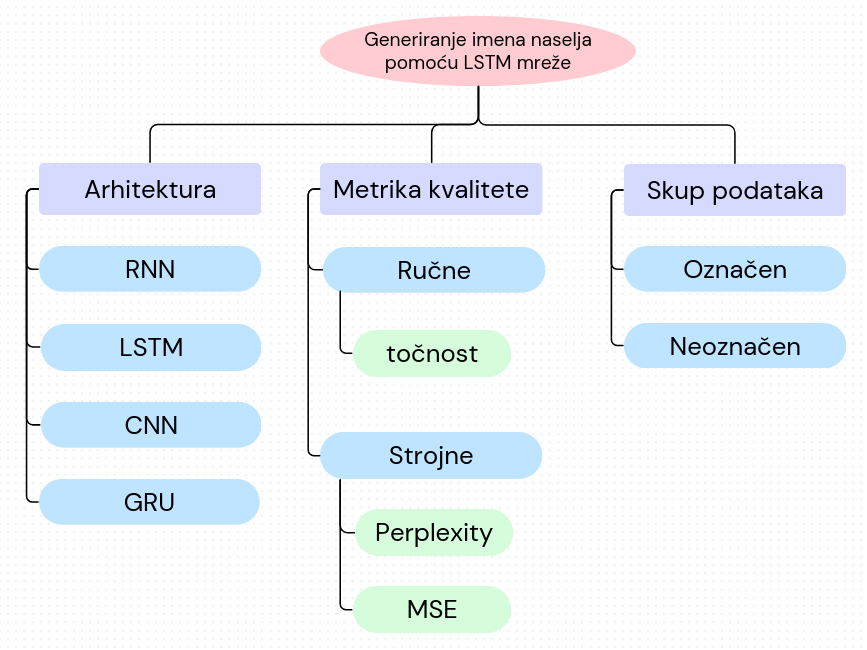
\includegraphics[angle=90, scale=0.3]{./pics/taksonomija3.png}\\
\caption{taksonomija rješenja za generiranje teksta}
\label{pic:takso}
\end{figure}

Nas samo zanimaju radovi na jezicima spomenutim u cjelini \ref{sect:intro} na razini riječi sa primjenom generiranja jezičnih konstrukta.\\
U konačnici odabiremo karakteristike našeg rješenja, navedene u tablici \ref{tab:hiper}.\\
\\
Nakon pretraživanja ukupno smo pronašli 9 relevantnih radova sa tražilica:
\begin{enumerate}
\item Google (5 radova)
\item IEEE Xplore (2 rada)
\item pretraživanje literature (2 rada)
\end{enumerate}

\begin{table}[H]
\caption{detalji pretraživanja}
\begin{center}
\begin{tabular}{|p{50pt}|p{110pt}|p{70pt}|}
\hline
 & & \textbf{Komentar}\\ \hline
tražilice & Google, Google Scholar, BASE, CORE, Science.gov, Semantic Scholar, Baidu scholar, RefSeek, CiteSeerX, ScienceOpen, The Lens, arXiv, AMiner, ACM, IEEE Xplore, Science Direct,  Springer Link, Web of Science & Samo smo na tražilici Google našli relevatne radove (njih 5)  \\ \hline
traženi pojam & (LSTM OR GRU OR CNN OR RNN OR Neural Network) AND ((~city AND ~generator AND ~name) OR (~generator AND ~name)) & Napisan sintaksom i operatorima koje koristi Google, ali na ostalim tražilicama je korišten prilagođeni izraz.\\ \hline
\end{tabular}
\label{tab:search}
\end{center}
\end{table}

Iako je problem kao takav složen (vidi poglavlje \ref{sect:zakljucak}), njegova izvedba je relativno jednostavna i teško primjenjiva na probleme u stvarnom svijetu te je zbog toga dostupno jako malo literature, koja je isključivo ograničena na hobi-projekte (\cite{master_LSTM}, \cite{name_generator}, \cite{data_name_generator}, \cite{city_name_gen}) i projekte u sklopu fakultetskih kolegija (\cite{randolph}, \cite{unreasonable_eff_of_LSTM}).\\




\section{Opis implementirane LSTM mreže}
Fokus projekta je treniranje i razvijanje neuronske mreže za generiranje realističnih imena naselja na različitim jezicima. Ukupno je dostupno generiranje imena na 5 jezika: engleski, francuski, hrvatski, španjolski, njemački. Moguće je generiranje toponima iz 7 različitih država (dodatno, SAD i Kanada). Korištenjem LSTM mreže, koja je prilagođena za analizu sekvencijskih podataka, cilj je razviti model sposoban za učenje jezičnih obrazaca i struktura iz postojećih imena naselja. Svrha mreže je generiranje novih imena temeljenih na tim naučenim obrascima, pri čemu se zadržavaju jezične i strukturne zakonitosti specifične za taj kontekst.\\
\\
Nadalje uz ćeliju je dodatno razvijeno GUI sučelje koje ima mogućnost generiranja 25 različitih imena gradova na 6 dostupnih jezika.\\
Težine jednom naučene mreže se pohranjuju u trajnu memoriju, odnosno u datoteke u za to predviđenom direktoriju: $\mathtt{./saved\_models}$.

\subsection{Arhitektura} \label{subsect:arh}
Arhitektura „LSTM“ mreže se sastoji od više ćelija koji omogućavaju propagaciju podataka na način da uz svako propagiranje ažuriraju se dugoročna i kratkotrajna memorija. Ideja je da struktura omogućava ćelijama da „pamte“ informacije kroz duže sekvence. Na slikama je prikazana LSTM ćelija kako je izvedena u radnom okviru keras.\\
Obično se više jedinica u sloju povezuje kao na slici \ref{tikz:vise_celija}, kao što je to slučaj kod Dense slojeva u našoj mreži. Međutim, isto ne vrijedi za LSTM jedinice.

\begin{figure}[H]
\centering
\subfigure[više jedinica općenito]{
	\label{tikz:vise_celija}
	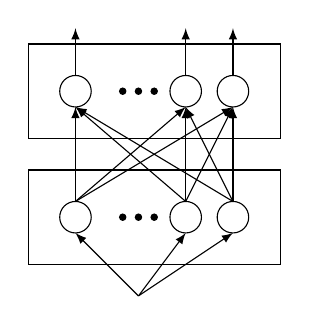
\begin{tikzpicture}[scale=0.4]
	\draw[draw=black, thin, solid] (-4.00,-1.00) rectangle (4.00,2.00);
	\draw[draw=black, thin, solid] (-2.50,0.50) ellipse (0.50 and 0.50);
	\draw[draw=black, thin, solid] (2.50,0.50) ellipse (0.50 and 0.50);
	\draw[draw=black, fill=black, thin, solid] (-1.00,0.50) circle (0.1);
	\draw[draw=black, fill=black, thin, solid] (-0.50,0.50) circle (0.1);
	\draw[draw=black, fill=black, thin, solid] (0.00,0.50) circle (0.1);
	\draw[draw=black, thin, solid] (-4.00,3.00) rectangle (4.00,6.00);
	\draw[draw=black, thin, solid] (-2.50,4.50) ellipse (0.50 and 0.50);
	\draw[draw=black, thin, solid] (2.50,4.50) ellipse (0.50 and 0.50);
	\draw[draw=black, fill=black, thin, solid] (-1.00,4.50) circle (0.1);
	\draw[draw=black, fill=black, thin, solid] (-0.50,4.50) circle (0.1);
	\draw[draw=black, fill=black, thin, solid] (0.00,4.50) circle (0.1);
	\draw[draw=black, -latex, thin, solid] (-0.50,-2.00) -- (-2.50,0.00);
	\draw[draw=black, -latex, thin, solid] (-0.50,-2.00) -- (2.50,0.00);
	\draw[draw=black, -latex, thin, solid] (-2.50,1.00) -- (2.50,4.00);
	\draw[draw=black, -latex, thin, solid] (2.50,1.00) -- (-2.50,4.00);
	\draw[draw=black, -latex, thin, solid] (-2.50,1.00) -- (-2.50,4.00);
	\draw[draw=black, -latex, thin, solid] (2.50,1.00) -- (2.50,4.00);
	\draw[draw=black, -latex, thin, solid] (-2.50,5.00) -- (-2.50,6.50);
	\draw[draw=black, -latex, thin, solid] (2.50,5.00) -- (2.50,6.50);
	\draw[draw=black, fill=white, thin, solid] (1.00,4.50) ellipse (0.50 and -0.50);
	\draw[draw=black, fill=white, thin, solid] (1.00,0.50) ellipse (0.50 and -0.50);
	\draw[draw=black, -latex, thin, solid] (2.50,1.00) -- (1.00,4.00);
	\draw[draw=black, -latex, thin, solid] (-0.50,-2.00) -- (1.00,0.00);
	\draw[draw=black, -latex, thin, solid] (1.00,1.00) -- (1.00,4.00);
	\draw[draw=black, -latex, thin, solid] (1.00,1.00) -- (2.50,4.00);
	\draw[draw=black, -latex, thin, solid] (1.00,1.00) -- (-2.50,4.00);
	\draw[draw=black, -latex, thin, solid] (-2.50,1.00) -- (1.00,4.00);
	\draw[draw=black, -latex, thin, solid] (1.00,5.00) -- (1.00,6.50);
\end{tikzpicture}
}
\subfigure[više LSTM jedinica]{
	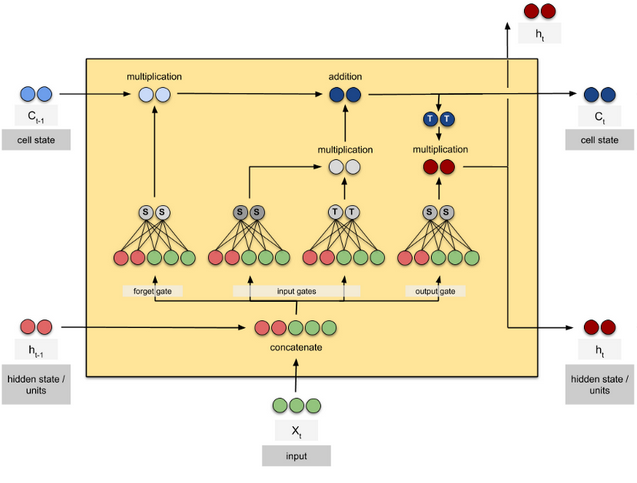
\includegraphics[scale=0.4]{./pics/lstm_jedinice.png}
	\label{subfig:lstm_cell_units}
}
\caption{ }
\end{figure}

Kao što vidimo na slici \ref{subfig:lstm_cell_units}, parametar \texttt{units=} keras klase \texttt{LSTM} upravlja dimenzijama svih vektora osim ulaznog. Keras LSTM sloj se ne sastoji od više povezanih LSTM ćelija, već od jedne LSTM ćelije kojoj je povećana dimenzionalnost izlaznog prostora te vektora koji upravljaju stanjem ćelije.
\ \\
U cjelini \ref{sect:intro} je opisan konceptualni izgled mreže: njena najjednostavnija varijanta (slika \ref{subfig:concept_cell}). Iz praktičnih razloga, implementacija izgleda nešto drugačije (slika \ref{subfig:real_cell}).

\begin{figure}[H]
\centering
\subfigure[Konceptualna arhitektura LSTM ćelije]{
		\label{subfig:concept_cell}
		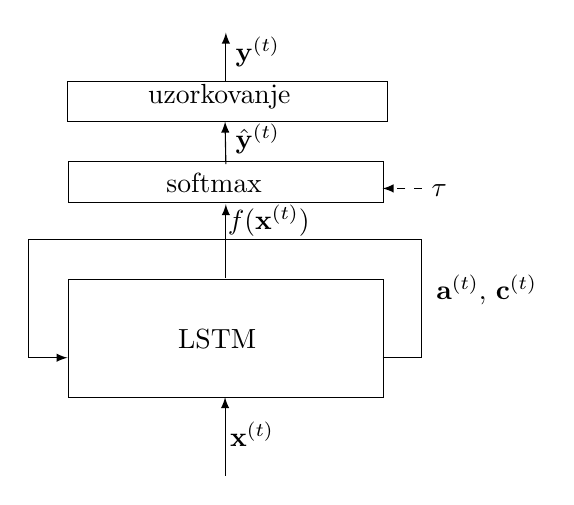
\begin{tikzpicture}
			\draw[draw=black, thin, solid] (-2.99,5.49) rectangle (1.01,4.00);
			\node[black, anchor=south west] at (-1.72,4.49) {LSTM};
			\draw[draw=black, -latex, thin, solid] (-1.00,3.00) -- (-1.00,4.00);
			\draw[draw=black, -latex, thin, solid] (-0.99,5.51) -- (-0.99,6.45);
			\draw[draw=black, thin, solid] (1.00,4.50) -- (1.50,4.50);
			\draw[draw=black, thin, solid] (1.50,4.50) -- (1.50,6.00);
			\draw[draw=black, thin, solid] (1.50,6.00) -- (-3.50,6.00);
			\draw[draw=black, thin, solid] (-3.50,6.00) -- (-3.50,4.50);
			\draw[draw=black, -latex, thin, solid] (-3.50,4.50) -- (-3.00,4.50);
			\draw[draw=black, thin, solid] (-2.99,6.99) rectangle (1.01,6.47);
			\draw[draw=black, -latex, thin, dashed] (1.5,6.65) -- (1.0,6.65);
			\node[black, anchor=south west] at (-1.87,6.47) {softmax};
			\node[black, anchor=south west] at (-0.99,6.96) {$\hat{\mathbf{y}}^{(t)}$};
			\node[black, anchor=south west] at (-1.06,3.25) {$\mathbf{x}^{(t)}$};
			\node[black, anchor=south west] at (-1.09,5.92) {$f(\mathbf{x}^{(t)})$};
			\draw[draw=black, -latex, thin, solid] (-0.99,6.96) -- (-1.00,7.50);
			\draw[draw=black, thin, solid] (-3.00,7.50) rectangle (1.06,8.01);
			\node[black, anchor=south west] at (-2.10,7.54) {uzorkovanje};
			\node[black, anchor=south west] at (-0.99,8.07) {$\mathbf{y}^{(t)}$};
			\draw[draw=black, -latex, thin, solid] (-0.99,8.02) -- (-0.99,8.63);
			\node[black, anchor=south west] at (1.56,5.05) {$\mathbf{a}^{(t)}$, $\mathbf{c}^{(t)}$};
			\node[black, anchor=south west] at (1.5,6.42) {$\tau$};
		\end{tikzpicture}
}
\subfigure[stvarna arhitektura LSTM mreže]{
	\label{subfig:real_cell}
	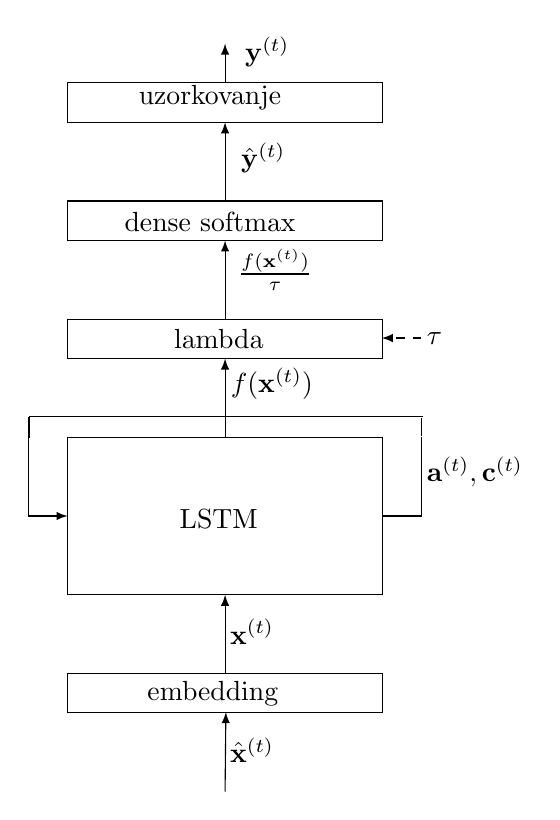
\begin{tikzpicture}
		\draw[draw=black, thin, solid] (-2.00,2.00) rectangle (2.00,0.00);
		\draw[draw=black, thin, solid] (-2.00,-1.00) rectangle (2.00,-1.50);
		\draw[draw=black, thin, solid] (-2.00,3.00) rectangle (2.00,3.50);
		\draw[draw=black, thin, solid] (-2.00,4.50) rectangle (2.00,5.00);
		\draw[draw=black, -latex, thin, solid] (0.00,-1.00) -- (0.00,0.00);
		\draw[draw=black, -latex, thin, solid] (0.00,2.00) -- (0.00,3.00);
		\draw[draw=black, -latex, thin, solid] (0.00,3.50) -- (0.00,4.50);
		\draw[draw=black, thin, solid] (-2.00,6.00) rectangle (2.00,6.50);
		\draw[draw=black, -latex, thin, solid] (0.00,5.00) -- (0.00,6.00);
		\draw[draw=black, -latex, thin, solid] (-2.50,1.00) -- (-2.00,1.00);
		\draw[draw=black, thin, solid] (2.00,1.00) -- (2.50,1.00);
		\draw[draw=black, thin, solid] (2.50,1.00) -- (2.50,2.00);
		\draw[draw=black, thin, solid] (-2.50,1.00) -- (-2.50,2.00);
		\draw[draw=black, thin, solid] (2.50,2.01) -- (2.50,2.25);
		\draw[draw=black, thin, solid] (-2.49,1.99) -- (-2.49,2.26);
		\draw[draw=black, thin, solid] (-2.49,2.26) -- (2.51,2.26);
		\node[black, anchor=south west] at (-0.70,0.72) {LSTM};
		\node[black, anchor=south west] at (-1.11,-1.53) {embedding};
		\node[black, anchor=south west] at (-0.77,3.00) {lambda};
		\node[black, anchor=south west] at (-1.40,4.49) {dense softmax};
		\node[black, anchor=south west] at (-1.22,6.03) {uzorkovanje};
		\draw[draw=black, -latex, thin, solid] (0.00,6.50) -- (0.00,7.00);
		\draw[draw=black, -latex, thin, dashed] (2.49,3.26) -- (1.99,3.26);
		\node[black, anchor=south west] at (2.44,3.05) {$\tau$};
		\draw[draw=black, -latex, thin, solid] (0.00,-2.50) -- (0.01,-1.49);
		\node[black, anchor=south west] at (-0.06,-2.25) {$\hat{\mathbf{x}}^{(t)}$};
		\node[black, anchor=south west] at (-0.06,-0.75) {$\mathbf{x}^{(t)}$};
		\node[black, anchor=south west] at (2.44,1.25) {$\mathbf{a}^{(t)}, \mathbf{c}^{(t)}$};
		\node[black, anchor=south west] at (-0.05,2.36) {$f(\mathbf{x}^{(t)})$};
		\node[black, anchor=south west] at (0.04,3.74) {$\frac{f(\mathbf{x}^{(t)})}{\tau}$};
		\node[black, anchor=south west] at (0.08,5.23) {$\hat{\mathbf{y}}^{(t)}$};
		\node[black, anchor=south west] at (0.13,6.58) {$\mathbf{y}^{(t)}$};
	\end{tikzpicture}
}
\caption{ }
\end{figure}


\subsection{Hipeparametri} \label{subsect:hiper}

\subsubsection{Dimenzija ulaznog vektora}
Dimenzija izlaznog vektora embedding sloja. Očekujemo $ \lvert \hat{\mathbf{x}} \rvert =  \lvert \Sigma \rvert$

\subsubsection{Dimenzija skrivenog stanja}
U trenutku $t$ sadrži informacije iz koraka $\{t-1, ..., 0\}$, stoga očekujemo monotono padajuću funkciju gubitka u ovisnosti o $\lvert \mathbf{a} \rvert$.

\subsubsection{Stopa učenja}
Koristimo ADAM optimizator, koji se temelji na stohastičkom gradijentnom spustu, stoga stopa uravlja numeričkom stabilnosti optimizacije. Očekujemo konveksnu funckiju: prevelike stope učenja dovode do nestabilnosti, a premale se presporo miču prema optimumu. (vidi \ref{subsect:trening})

\subsubsection{Temperatura}
\begin{figure}[H]
\begin{equation}
\sigma_{\tau}(\mathbf{f_i}) = \frac{e^{\mathbf{f}_i/\tau}}{\sum_{j=0}^{\lvert f \rvert} e^{\mathbf{f}_j/\tau} }
\end{equation}
\caption{Temperaturni softmax}
\end{figure}

temperaturom parametrizirani softmax čuva poredak vjerojatnosti klasa, ali smanjuje razliku između njih:
\begin{equation}
\mathbf{f}_i \geq \mathbf{f}_j \implies \sigma_{\tau}(\mathbf{f}_i) \geq \sigma_{\tau}(\mathbf{f}_j)
\end{equation}

\begin{equation}
\mathbf{f}_i - \mathbf{f}_j \geq \sigma_{\tau}(\mathbf{f}_i) - 
 \sigma_{\tau}(\mathbf{f}_j)
\end{equation}
Što za izravnu posljedicu ima jednolikiji izbor konačnih klasa, odnosno "kretivniji" ispis, kada $\tau > 1$, odnosno "predvidljiviji" ispis kada $\tau < 1$.



\begin{table}[htbp]
\caption{hiperparametri naše mreže}
\begin{center}
\begin{tabular}{|p{120pt}|p{40pt}|p{60pt}|}
\hline
\textbf{Hiperparametar} & \textbf{\textit{Vrijednost}} & \textbf{\textit{komentar}}\\ \hline
%broj jedinica po sloju &  & Broj jedinica po sloju određuje, između ostalog, i dimenziju skrivenog stanja ($\lvert \mathbf{a} \rvert$). (vidi \ref{subsect:arh})\\ \hline
temperatura ($\tau$) &  & Daje mogućnost upravljanja "kreativnošću" generiranje. \\ \hline
dimenzija izlaznog prostora embedding sloja ($\lvert \mathbf{x} \rvert$) &  & \\ \hline
dimenzija skrivenog stanja ($\lvert \mathbf{a} \rvert$) &  & \\   \hline
stopa učenja ($\mu$) &  & \\ \hline \hline
aktivacijska funckija & $\tanh$ & zadano \\ \hline
povratna akt. funkcija & $\sigma$ & zadano \\ \hline
bias & da & zadano \\ \hline
inicijalizator kernela & glorot jednoliki & zadano \\ \hline
inicijalizator povratne veze & glorot jednoliki & zadano \\ \hline
bias inicijalizator & zeros & zadano \\ \hline
forget bias & da & zadano \\ \hline
regularizacija kernela & & zadano \\ \hline
regularizacija kernela povratne veze &  & zadano \\ \hline
bias regularizacija &  & zadano \\ \hline
kernel ograničenje &  & zadano \\ \hline
povratno ograničenje &  & zadano \\ \hline
bias ograničenje & & zadano\\ \hline
dropout & 0 & zadano \\ \hline
povratni dropout & 0 & zadano \\ \hline
\end{tabular}
\label{tab:hiper}
\end{center}
\end{table}


\subsection{Ćelija}
Ćelije su najbitniji dio naše mreže. Osim ulaza i izlaz ćelije imaju dugoročnu $\mathbf{c}$ i kratkoročnu memoriju $\mathbf{a}$. Ti su vektori svojstveni za ovakav tip mreže i razlikuju je od drugih RNN. Slika \ref{tikz:detail} prikazuje unutarnju shemu ćelije, $[\quad, \quad]$ označava operaciju konkatenacije.
\ \\
Vidimo njene sastavne dijelove:
\begin{table}[htbp]
\caption{hiperparametri naše mreže}
\begin{center}
\begin{tabular}{|p{80pt}|p{140pt}|}
\hline
\textbf{Komponenta} & \textbf{\textit{komentar}}\\ \hline
ulazni vektor $\mathbf{x}$ & \\ \hline
izlazni vektor $\mathbf{y}$ & \\ \hline
kratkoročna memorija $\mathbf{a}$ & Kratkoročna memorija ili skriveno stanje, povezano težinskim vezama sa drugim komponentama, može se modificirati. \\ \hline
dugoročna memorija $\mathbf{c}$ & Iako se dugoročna memorija može modificirati množenjem, a zatim kasnije zbrajanjem, ne postoje težine i bias koji mogu izravno modificirati memoriju. Nedostatak težina omogućuje dugoročnim sjećanjima da teku kroz niz odmotanih jedinica bez nestanka ili beskonačnog gradijenta. \\ \hline
Memorijski sklop & Specifičnost je da se kombiniraju ulaz i kratkoročna memorija pomnoženi sa prikladnim težinama te na kraju se dodaje bias. Ta funkcija prolazi kroz sigmoidnu aktivacijsku funkciju koja na kraju se množi sa dugoročnom memorijom. Ako je $\sigma( [\mathbf{x}^{(t)}, \mathbf{a}^{(t)}] \cdot W_f + b_f) \approx 1 $ pamtimo puno te $\mathbf{c}^{(t)}$ ostaje skoro nepromijenjen. U suprotnom ako je gornji izraz $\approx 0$ dolazi do velike numeričke promjene (poništavanja). \\ \hline
Ulazni sklop &  Vrijednost $\sigma( [\mathbf{x}^{(t)}, \mathbf{a}^{(t)}] \cdot W_i + b_i)$ stvara potencijalno dugoročno sjećanje, a vrijednost $\tanh( [\mathbf{x}^{(t)}, \mathbf{a}^{(t)}] \cdot W_m + b_m)$ određuje koji postotak tog sjećanja će se zapamtiti. \\ \hline
Izlazni sklop & Kombiniramo novostvorenu dugoročnu memoriju $\tanh(\mathbf{c}^{(t+1)})$ sa rezutatom sigmoide koji odlučuje u kojoj mjeri će se zapamtiti novostvoreno sjećanje. Na izlazu dobivamo novo kratoročno sjećanje, odnosno izlazni vektor $f(\mathbf{x}^{(t)})$ (slično kao ulazni sklop) \\ \hline
\end{tabular}
\label{tab:hiper}
\end{center}
\end{table}

U teoriji modeli neuronskih mreža u kerasu mogu raditi sa ulaznim vektorima varijabilne dimenzionalnosti. U praksi, rad sa vektorima fiksne duljine poboljšava performanse, osobito vrijeme treniranja. Razlog tomu je to što ulazni vektori fiksne težine omogućavaju stvaranje tenzora fiksnih oblika, a posljedično i stabilne težine.\\



\subsection{Treniranje} \label{subsect:trening}
BPTT je korišten kao algoritam učenja.
Kao funkcija gubitka koristi se kategorička unakrsna entropija.
\begin{equation}
L = - \sum_{t = 0}^{\lvert \Sigma \rvert-1} \mathbf{z}_i^{(t)} \cdot log(\hat{\mathbf{y}}_i^{(t)})
\end{equation}
Gdje je $i \in [0, \lvert \Sigma \rvert - 1]$. $\hat{\mathbf{y}}^{(t)}$ je izlaz mreže, odnosno $\hat{\mathbf{y}}_i^{(t)}$ vjerojatnost da je idući znak $i$-ti znak abecede, a $\mathbf{z}^{(t)}$ je očekivani vektor.
Inačica BPTT koju mi koristimo je u biti propagirani stohastički gradijentni spust.\\
\\
Pri treniranju koristimo parametre navedene u tablici \ref{tab:trening}.
\begin{table}[htbp]
\caption{parametri procedure za treniranje}
\begin{center}
\begin{tabular}{|c|c|}
\hline
\textbf{Parametar} & \textbf{\textit{Vrijednost}}\\ \hline
f-ja gubitka & kategorička unakrsna entropija \\ \hline
algoritam optimizacije & ADAM \\ \hline
metrika kvalitete & točnost \\ \hline
\end{tabular}
\label{tab:trening}
\end{center}
\end{table}

Pri treniranju koristimo podjelu skupova na skup za treniranje i testiranje (validaciju) u omjeru 4:1.\\
Uz hiperparametre $\begin{bmatrix} \lvert \mathbf{a} \rvert & \mu & \lvert \mathbf{\hat{x}} \rvert & \tau \end{bmatrix} = \begin{bmatrix} 128 & 10^{-3} & 100 & 0.004885  \end{bmatrix}$ dobivamo slijedeće vrijednosti funkcije gubitka i točnosti po epohama.\\
\\
Zbog ograničenja sa skupovima podataka te kako bi se omogućila usporedba veličina skupa za testiranje svih jezika je ograničena na $\lvert \mathcal{D}_{test, L} \rvert = \min_{L} \lvert \mathcal{D}_{test, L} \rvert = \lvert \mathcal{D}_{test, GER} \rvert \approx 600$.


\begin{figure}[H]
\centering
\subfigure{
	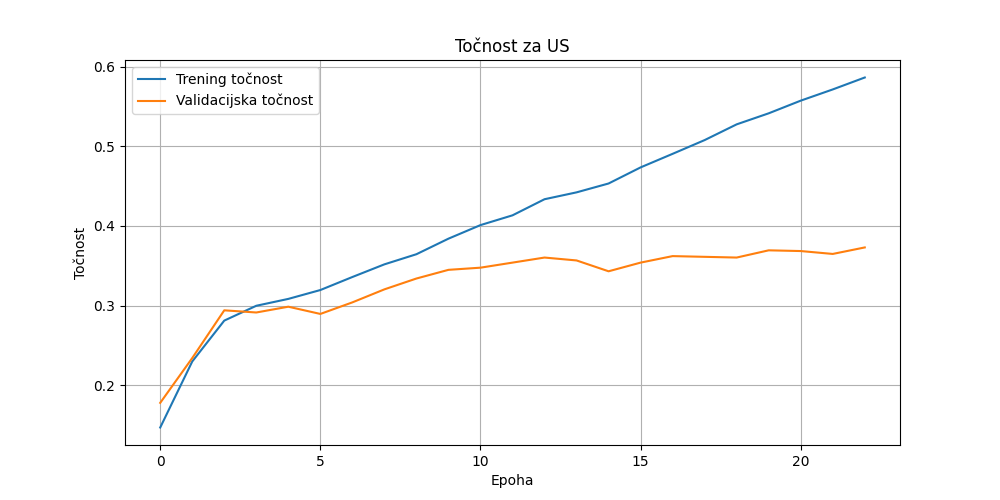
\includegraphics[scale=0.4]{../saved_models/US_accuracy_plot.png}
}
\subfigure{
	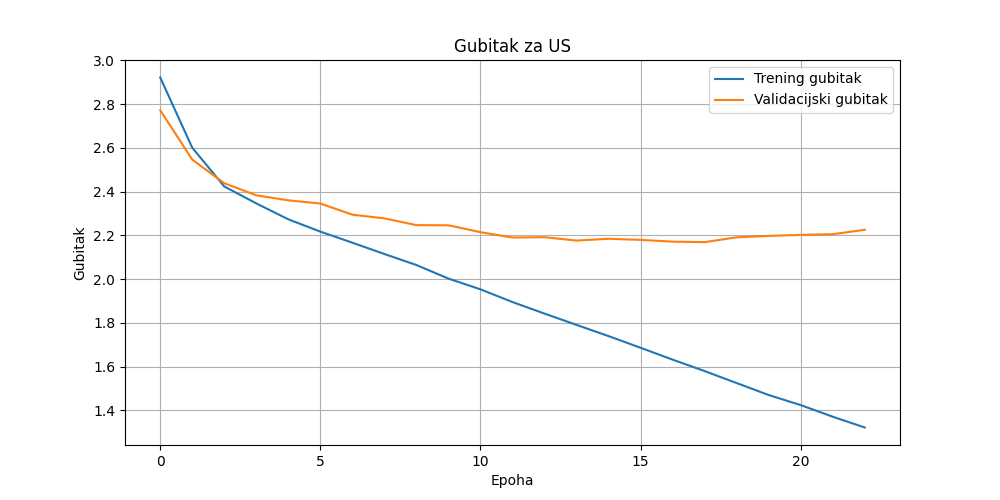
\includegraphics[scale=0.4]{../saved_models/US_loss_plot.png}
}
\caption{Američki gradovi}
\end{figure}
Grafovi za ostale jezike izgledaju gotovo identično, greška na skupu za testiranje počinje rasti nakon 20-30 epohe. Najveća točnost je uvijek $40\% \pm 5\%$.

\section{Opis eksperimentalnih rezultata} 
\subsection{optimiranje hiperparametara}
Optimiranje je izvršeno strojno, pomoću razreda \texttt{GridSearch}.
Pokrenut je automatski postupak optimizacije nad 4 hiperparametra naše mreže, te su dobivene vrijednosti $\mathbf{\boldsymbol{\theta}_m} = \begin{bmatrix} \lvert \mathbf{x} \rvert_m & \lvert \mathbf{a} \rvert_m & \mu_m & \tau_m \end{bmatrix} = \begin{bmatrix} 32 & 224 & 0.00406 & 0.00802 \end{bmatrix}$.
Vrijednosti optimuma $E[L(\mathbf{\boldsymbol{\theta}}_m) | \mathcal{D}_{test}] = 2.229$.\\
\\
Vidimo da su naša predviđanja iz cjeline \ref{subsect:hiper} bila većinom točna, sa iznimkom onog za skriveno stanje $\lvert \mathbf{a} \rvert$: nije riječ o monotono padajućoj funkciji pogreške u ovisnosti o tom hiperparametru, već o konveksnoj. Razlog tomu je moguće to što je riječ o kratkim nizovima znakova za koje postoji ograničena količina informacija koja se ima za zapamtiti između vremenskih koraka.

\subsection{Usporedba rezultata}
U tablici dajemo kratku usporedbu sa rezultatima u literaturi.
Kao i u prethodnom cjelinama, korišten je skup podataka Američkih gradova (skup koji ima najmanju točnost na skupu za validaciju).
\begin{table}[H]
\caption{ }
\begin{center}
\begin{tabular}{|c|c|c|c|}
\hline
 & \textbf{\cite{randolph}} & \textbf{\cite{name_generator}} & \textbf{Naša mreža}  \\ \hline
\textbf{točnost} & $40\%$ & $40\%^{\mathrm{a}}$ &  \\ \hline
\multicolumn{4}{l}{$^{\mathrm{a}}$at optimal $\tau=0.5$.}
\end{tabular}
\label{tab:result}
\end{center}
\end{table}
%Mrežu smo pokrenuli nad uzorkom od $(N= 10, n=25)$ pokretanja, odnosno imena te dobili rezultat i interval povjerenja $(\alpha= 0.95, \nu= 9)$ u gornjoj tablici.

Vrijedi napomenuti da, zbog svojstvenosti problema, točnost na ispitnom skupu predstavlja donju granicu stvarne točnosti modela. Naime moguće je da:
\begin{enumerate}
\item U skupu za ispitivanje postoje gradovi koji nisu u skupu za testiranje, a postoje u stvarnosti.
\item U skupu za ipistivanje postoje realistični, ali nepostojeći gradovi (cilj zadatka)
\end{enumerate}
Budući da $\lvert \mathcal{D} \rvert \approx 600$, prva točka je vrlo izgledna. Stoga $E[L(\mathbf{\boldsymbol{\theta}}_m) | \mathcal{D}_{test}]$ podcjenuje mogućnost generalizacije našeg modela.

\section{Zaključak} \label{sect:zakljucak}
Krajnji rezultat je mreža koja ima željenu točnost $\eta \approx 0.4$, svi projekti navedeni u literaturi dobivaju istu vrijednosti točnosti. Mišljenje je autora da je uzrok tako niskoj točnosti u samom problemu. Naime, iako su u toponimima uočljivi obrasci, također je prisutna velika raznolikost među imenima. Predviđanje realističnih imena je, stoga, izazovan zadatak.\\
Nije moguće proširiti skup podataka ta učenje, jer su svi postojeći gradovi već navedeni u skupu za učenje. Također je malo vjerojatno da će se na točnosti dobiti tako da se promijeni arhitektura mreže i/ili ćelije, jer je LSTM više nego dovoljno složena arhitektura za generiranje kratkih nizova znakova.\\
Kao moguće rješenje autori predlažu proširenje izvornog skupa podataka za učenje gradovima koji ne postoje. To se može ostvariti na bilo kojim, ili kombinacijom ova dva pristupa:
\begin{enumerate}
\item ručno: ljudi izmišljaju imena gradova te osiguravaju da već ne postoje.
\item strojno: LSTM mreža generira imena gradova, te pohranjuje u idući skup za učenje one nazive koji već ne postoje.
\end{enumerate}

Ako pitamo ChatGpt 4 da generira 25 imena američkih gradova on to radi sa $80\%$ točnosti međutim većina tih gradova je u skupu za učenje (CommonCrawl ili OpenWebText najvjerojatnije), a oni koji nisu su vrlo slični njima. Autori vjeruju da je upravo to razlog visokoj točnosti GPT te da bi takav pristup, implementiran na prethodno opisan način, znatno poboljšao točnost naše mreže.




\begin{thebibliography}{00}
\bibitem{Fatima} Fatima, N., Imran, A S., Kastrati, Z., Daudpota, S M., Soomro, A (2022) ``A Systematic Literature Review on Text Generation Using Deep Neural Network Models``
IEEE Access, 10: 53490-53503, https://doi.org/10.1109/ACCESS.2022.3174108
\bibitem{hyper_choise_1} Eckhardt K. (2018, November 29). Choosing the right Hyperparameters for a simple LSTM using Keras. Towards data science. https://towardsdatascience.com/choosing-the-right-hyperparameters-for-a-simple-lstm-using-keras-f8e9ed76f046
\bibitem{unreasonable_eff_of_LSTM} Karpathy A. (2015, May 21). The Unreasonable Effectiveness of Recurrent Neural Networks. Andrej Karpathy blog. http://karpathy.github.io/2015/05/21/rnn-effectiveness
\bibitem{randolph} Randolph Z. (2020.) ``Recursive Neural Network for Generating Novel
Brand Names for Therapeutic Medicines``. report. Department of Computer Science. Stanford. http://cs230.stanford.edu/projects\_spring\_2020/reports/38912979.pdf
\bibitem{unreasonable_eff_of_LSTM} Olah C. (2017, August 27). Understanding LSTM Networks. colah's blog. https://colah.github.io/posts/2015-08-Understanding-LSTMs/
\bibitem{master_LSTM} Dipanshu G. (2017, August 27). Master LSTM Networks With Python: A Guide Using TensorFlow and Keras. Medium. https://dipanshu10.medium.com/implementing-lstm-networks-with-python-a-guide-using-tensorflow-and-keras-915b58f502ce
\bibitem{name_generator} Rahalkar C. (2019, June 29). Name Generator Using Recurrent Neural Networks. Github. https://github.com/chaitanyarahalkar/Name-Generator-RNN
\bibitem{data_name_generator} Landy C. (2019, September 7). Look No More, The Data driven Baby Name generator. www.connorlandy.com. https://www.connorlandy.com/projects/rnn-name-generator
\bibitem{city_name_gen} Bosnali C. (2018, September 27). City-Name-Generation-using-LSTM-and-TF. Github. https://github.com/CihanBosnali/City-Name-Generation-using-LSTM-and-TF
\end{thebibliography}



\begin{sidewaysfigure*}
\label{tikz:detail}
\resizebox{550pt}{!}{
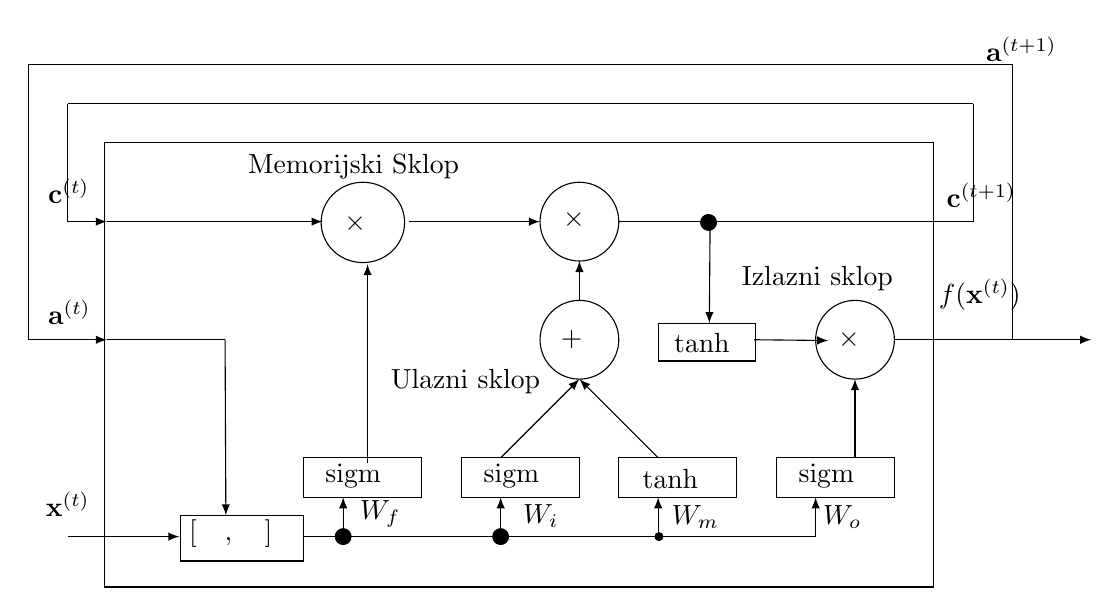
\begin{tikzpicture}
	\draw[draw=black, thin, solid] (-5.03,0.86) rectangle (5.50,6.50);
	\draw[draw=black, thin, solid] (4.50,4.00) ellipse (0.50 and -0.50);
	\draw[draw=black, thin, solid] (1.00,4.00) ellipse (0.50 and -0.50);
	\draw[draw=black, thin, solid] (1.00,5.50) ellipse (0.50 and -0.50);
	\draw[draw=black, thin, solid] (-1.75,5.49) ellipse (0.53 and 0.51);
	\draw[draw=black, thin, solid] (1.50,2.00) rectangle (3.00,2.50);
	\draw[draw=black, thin, solid] (-0.50,2.50) rectangle (1.00,2.00);
	\draw[draw=black, thin, solid] (-2.50,2.00) rectangle (-1.00,2.50);
	\draw[draw=black, thin, solid] (-4.07,1.77) rectangle (-2.50,1.19);
	\draw[draw=black, thin, solid] (3.50,2.00) rectangle (5.00,2.50);
	\node[black, anchor=south west] at (2.08,3.72) {tanh};
	\node[black, anchor=south west] at (1.68,1.99) {tanh};
	\node[black, anchor=south west] at (-2.35,2.00) {sigm};
	\node[black, anchor=south west] at (3.66,1.99) {sigm};
	\node[black, anchor=south west] at (-0.34,1.99) {sigm};
	\node[black, anchor=south west] at (-4.08,1.24) {$[\quad , \quad]$};
	\node[black, anchor=south west] at (-1.52,3.19) {Ulazni sklop};
	\node[black, anchor=south west] at (2.94,4.50) {Izlazni sklop};
	\node[black, anchor=south west] at (-3.33,5.92) {Memorijski Sklop};
	\node[black, anchor=south west] at (-1.91,1.49) {$W_f$};
	\node[black, anchor=south west] at (0.16,1.49) {$W_i$};
	\node[black, anchor=south west] at (2.05,1.48) {$W_m$};
	\node[black, anchor=south west] at (3.97,1.48) {$W_o$};
	\node[black, anchor=south west] at (-5.87,4.07) {$\mathbf{a}^{(t)}$};
	\node[black, anchor=south west] at (6.04,7.41) {$\mathbf{a}^{(t+1)}$};
	\node[black, anchor=south west] at (5.54,5.55) {$\mathbf{c}^{(t+1)}$};
	\node[black, anchor=south west] at (-5.87,5.60) {$\mathbf{c}^{(t)}$};
	\node[black, anchor=south west] at (5.44,4.25) {$f(\mathbf{x}^{(t)})$};
	\node[black, anchor=south west] at (-5.90,1.63) {$\mathbf{x}^{(t)}$};
	\node[black, anchor=south west] at (-2.11,5.23) {$\times$};
	\node[black, anchor=south west] at (0.67,5.28) {$\times$};
	\node[black, anchor=south west] at (4.16,3.76) {$\times$};
	\node[black, anchor=south west] at (0.64,3.76) {$+$};
	\draw[draw=black, thin, solid] (2.00,3.73) rectangle (3.24,4.21);
	\draw[draw=black, -latex, thin, solid] (-1.69,2.44) -- (-1.69,4.96);
	\draw[draw=black, -latex, thin, solid] (-5.00,5.50) -- (-2.26,5.50);
	\draw[draw=black, -latex, thin, solid] (-1.17,5.50) -- (0.50,5.50);
	\draw[draw=black, -latex, thin, solid] (1.00,4.50) -- (1.00,5.00);
	\draw[draw=black, -latex, thin, solid] (0.00,2.50) -- (1.00,3.50);
	\draw[draw=black, -latex, thin, solid] (2.00,2.50) -- (1.00,3.50);
	\draw[draw=black, -latex, thin, solid] (-0.00,1.51) -- (0.00,2.00);
	\draw[draw=black, -latex, thin, solid] (2.00,1.50) -- (2.00,2.00);
	\draw[draw=black, -latex, thin, solid] (4.00,1.50) -- (4.00,2.00);
	\draw[draw=black, -latex, thin, solid] (-2.00,1.50) -- (-2.00,2.00);
	\draw[draw=black, thin, solid] (-2.50,1.50) -- (4.00,1.50);
	\draw[draw=black, fill=black, thin, solid] (2.01,1.50) ellipse (0.05 and -0.05);
	\draw[draw=black, -latex, thin, solid] (-5.50,1.50) -- (-4.08,1.50);
	\draw[draw=black, -latex, thin, solid] (3.22,4.00) -- (4.16,3.99);
	\draw[draw=black, -latex, thin, solid] (-5.50,5.50) -- (-5.00,5.50);
	\draw[draw=black, -latex, thin, solid] (-3.50,4.00) -- (-3.49,1.77);
	\draw[draw=black, -latex, thin, solid] (4.50,2.50) -- (4.50,3.50);
	\draw[draw=black, -latex, thin, solid] (2.66,5.51) -- (2.65,4.21);
	\draw[draw=black, fill=black, thin, solid] (-2.00,1.50) circle (0.1);
	\draw[draw=black, fill=black, thin, solid] (0.00,1.50) circle (0.1);
	\draw[draw=black, fill=black, thin, solid] (2.64,5.49) circle (0.1);
	\draw[draw=black, thin, solid] (5.00,4.00) -- (6.50,4.00);
	\draw[draw=black, thin, solid] (6.50,4.00) -- (6.50,7.50);
	\draw[draw=black, thin, solid] (6.50,7.50) -- (-6.00,7.50);
	\draw[draw=black, thin, solid] (-6.00,7.50) -- (-6.00,4.00);
	\draw[draw=black, -latex, thin, solid] (-6.00,4.00) -- (-5.00,4.00);
	\draw[draw=black, thin, solid] (-5.00,4.00) -- (-3.50,4.00);
	\draw[draw=black, -latex, thin, solid] (6.50,4.00) -- (7.50,4.00);
	\draw[draw=black, thin, solid] (1.50,5.50) -- (6.00,5.50);
	\draw[draw=black, thin, solid] (6.00,5.50) -- (6.00,7.00);
	\draw[draw=black, thin, solid] (6.00,7.00) -- (-5.50,7.00);
	\draw[draw=black, thin, solid] (-5.50,7.00) -- (-5.50,5.50);
\end{tikzpicture}
}
\caption{Unutarnja arhitektura LSTM ćelije}
\end{sidewaysfigure*}




\end{document}
